\documentclass[12pt]{article}
\usepackage{listings}
\usepackage{color}
\usepackage{amssymb}
\usepackage{amsmath}
% defining tab
\newcommand\tab[1][1cm]{\hspace*{#1}}
% \usepackage{graphicx}
% \usepackage{wrapfig}
% \graphicspath{ {images/} 

% defining the code thingy
\definecolor{codegreen}{rgb}{0,0.6,0}
\definecolor{codegray}{rgb}{0.5,0.5,0.5}
\definecolor{codepurple}{rgb}{0.58,0,0.82}
\definecolor{backcolour}{rgb}{0.95,0.95,0.92}

\lstdefinestyle{mystyle}{
    backgroundcolor=\color{backcolour},   
    commentstyle=\color{codegreen},
    keywordstyle=\color{magenta},
    numberstyle=\tiny\color{codegray},
    stringstyle=\color{codepurple},
    basicstyle=\footnotesize,
    breakatwhitespace=false,         
    breaklines=true,                 
    captionpos=b,                    
    keepspaces=true,                 
    numbers=left,                    
    numbersep=5pt,                  
    showspaces=false,                
    showstringspaces=false,
    showtabs=false,                  
    tabsize=2
}
\lstset{style=mystyle}

\begin{document}
\title{{\huge \bfseries Transportation Network Documentation}}
\author{Ormir Gjurgjej, Nitika Kumar}
\maketitle

\section{Introduction}
The first thing to consider when working with graphs is what type of graph you are working with. Here we have the Viennese public transportation network that clearly consists of more vertices (stations) than edges (connection between each vertex) which is why the implementation of an adjacency list has been more beneficial in our case rather than the use of an adjacency matrix. 
% For that we implemented a list with the so called "queue" by including the \textless queue\textgreater library.
\\
The aim of this program is to find the shortest path from a starting point to a destination using the Priority First Search as in Dijkstra's algorithm. The purpose of this documentation is to explain each step taken for the implementation of this algorithm making it possible for any user to calculate an overall travel time in order to reach a location from any starting point whereas both - start and finish - are completely arbitrary.\\
We started off by creating two classes - Network and Station. Each object of the second class which represents one station of the transportation network system is the vertex of the graph. The minutes inbetween stand for the edges that connect every vertex.\\
\section{Introducing the Datastructures}
\subsection{Station}
This class is responsible for the vertices of the entire graph. As the adjacency list requires us to do, each vertex contains the name of the station, the line it belongs to (either metro or tram) and a map which contains a reference to the neighbours (nodes) next to the current vertex that we are positioned on including the distance as in how long it takes to get there. The following code snippet shows the private members of the Station class $\colon$ \\

\begin{lstlisting}[language=C++, caption = class Station(private members)]
class Station {
    std::string name;
    std::string line;
    std::map<Station*, int> neighbours;
    ...
};
\end{lstlisting}

\noindent Furthermore this class contains several functions, a constructor and a destructor.\\
One of them is getDistance(). The distance from one vertex x to another vertex y can be defined as $\colon$
 
 \[d(x,y) =
 \begin{cases} \text{Min \{w(p) $|$ p is the way from x to y\} if a way exists}\\
                 \text{Infinite if no way exists}
\end{cases}
\]
\\
The infinite in our case is defined in the header file station.hpp as INF with the value 999 which means that if the name of the station and its distance are not found anywhere in the "neighbours" map, this function returns INF.

\begin{lstlisting}[language=C++, caption = getDistance()]
int Station::getDistance(Station* nStation) const {
    try {
        return neighbours.at(nStation);
    } catch (std::out_of_range e) {
        return INF;
    }
}
\end{lstlisting}

The info() function returns a beautiful output of the entire tranportation network that was imported by the user in the terminal. Each station is listed in an alphabetical order, here is a snippet $\colon$ \\

% \begin{wrapfigure}{r}
% 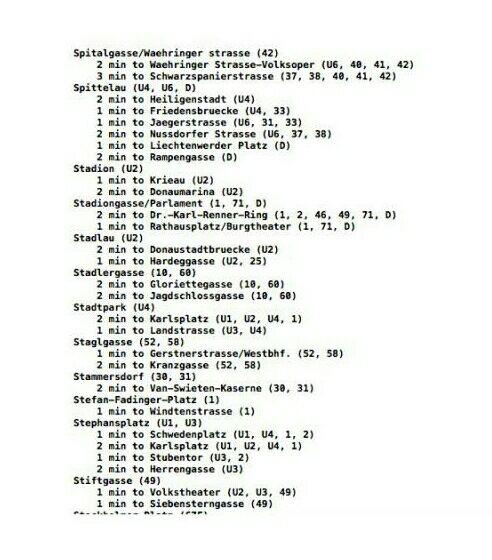
\includegraphics[width=11cm, height=11cm]{infotrans}
% In order to understand the purpose of all of these, I am going to introduce you to the class Network first.
% \end{wrapfigure}
\noindent Spittelau (U4, U6, D)\\
    \tab2 min to Heiligenstadt (U4)\\
    \tab1 min to Friedensbruecke (U4, 33)\\
    \tab1 min to Jaegerstrasse (U6, 31, 33)\\
    \tab2 min to Nussdorfer Strasse (U6, 37, 38)\\
    \tab1 min to Liechtenwerder Platz (D)\\
    \tab2 min to Rampengasse (D)\\
Stadion (U2)\\
    \tab1 min to Krieau (U2)\\
    \tab2 min to Donaumarina (U2)\\
Stadiongasse/Parlament (1, 71, D)\\
    \tab2 min to Dr.-Karl-Renner-Ring (1, 2, 46, 49, 71, D)\\
    \tab1 min to Rathausplatz/Burgtheater (1, 71, D)\\
Stadlau (U2)\\
    \tab2 min to Donaustadtbruecke (U2)\\
    \tab1 min to Hardeggasse (U2, 25)\\
Stadlergasse (10, 60)\\
    \tab2 min to Gloriettegasse (10, 60)\\
    \tab2 min to Jagdschlossgasse (10, 60)\\
Stadtpark (U4)\\
    \tab2 min to Karlsplatz (U1, U2, U4, 1)\\
    \tab1 min to Landstrasse (U3, U4)\\
Staglgasse (52, 58)\\
    \tab1 min to Gerstnerstrasse/Westbhf. (52, 58)\\
    \tab2 min to Kranzgasse (52, 58)\\
Stammersdorf (30, 31)\\
    \tab2 min to Van-Swieten-Kaserne (30, 31)\\
Stefan-Fadinger-Platz (1)\\
    \tab1 min to Windtenstrasse (1)\\
Stephansplatz (U1, U3)\\
    \tab1 min to Schwedenplatz (U1, U4, 1, 2)\\
    \tab2 min to Karlsplatz (U1, U2, U4, 1)\\
    \tab1 min to Stubentor (U3, 2)\\
    \tab2 min to Herrengasse (U3)\\


\begin{lstlisting}[language=C++, caption = info() displays the network]
void Station::info() {
    std::cout << name << " (" << line << ")" << std::endl;
    for (auto it = neighbours.begin(); it != neighbours.end(); ++it) {
        std::cout << '\t' << it->second << " min to " << it->first->getName() << " (" << it->first->getLine() << ")" << std::endl;
    }
}
\end{lstlisting}

\subsection{Network}
Network.cpp consists of functions that enable the user to ask for help (opening the README.txt file), to import a file of a transportation network by typing "import", to show all the stations and lines thanks to the info() function as well as executing the dijkstra algorithm by typing in "search" followed by the starting point and destination (calling the path() function).\\

\section{Dijkstra's Algorithm}
Perhaps the most difficult part of this project was the implementation of Dijkstra's algorithm. The reason why we used this algorithm and not Bellman-Ford's one is because the edges do not have a negative weight. It all takes place in Network's function called path() which takes two parameters - the name of the starting point and the name of the destination. You will find the entire code snippet below.\\
First, we ensure that the stations entered by the user are part of the network (ubahn.txt). If so, we move on to cmp that stores a condition that we will need for the priority queue afterwards. We used "pair" as a datatype as it stores two values $\colon$ a pointer pointing to the neighbour nodes (Station*) and the amount of time it takes to reach this station (int).\\
The good thing about priority queues as opposed to normal queues is that you can have a certain criterion for the order of the elements in the queue, which is defined in the "decltype(cmp)\textgreater queue(cmp);". This means that whenever the condition left.first\textgreater right.first (distance of left vertex greater than the distance of the right vertex) is true, add this element by first comparing it with each element in the priority queue and then pushing it in at the right place.\\
In order to keep an overview of the stations that were visited we used a \textless set\textgreater to store all the stations on the way from source to destination. We also created a \textless map\textgreater where we save the minutes/travel time each time we iterate over the vertices.\\
Here comes the defining part $\colon$ head is a pointer always pointing to the top element of the queue (as we used a priority queue, mentioned previously) or in other words, it is always the current position that we are located on between source and destination. Every time head moves over to the next station, the top element is first removed with the queue.pop() function. If head is not part of the visited stations (set) yet, insert it into the set. This process is repeated as long as head finishes iterating over every single element in the queue.\\ 
We then create another map called nbList and assign all the neighbours of head to it. Eventually, we need to iterate over each neighbour station and just check if the distance of the vertex has already been saved in the distance map. If the new distance (newDis) is shorter than the older distance (dist[nb-\textgreater first]), it is added to the map dist. newDis contains the distance from source to the current station and in addition to the neighbour. dist[nb-\textgreater first] however just stores the distance between source and any neighbour station. Finally, the distance variable is updated and adds together all the minutes it found along the shortest path between source and destination.\\
In order to display the path we iterate over the neighbours again but in reverse.  
\\
\begin{lstlisting}[language=C++, caption = Dijkstra's algorithm implemented in path()]
bool Network::path(std::string bName, std::string eName) {
        Station *source, *destination;
    try {
        source = stations.at(bName);
        destination = stations.at(eName);
    } catch (std::out_of_range e) {
        std::cout << "Couldn't find begin or end station" << std::endl;
        return false;
    }
    
    Station * head = source;
    
    auto cmp = [](std::pair<int, Station*> left, std::pair<int, Station*> right) {
        return left.first > right.first;
    };
    
    std::priority_queue<std::pair<int, Station*>, std::vector<std::pair<int, Station*>>,decltype(cmp)> queue(cmp);
    queue.push(std::make_pair(0, source));
    
    std::set<Station*> visited;
    std::map<Station*, int> dist;
    dist[source] = 0;
    
    while (!queue.empty()) {
        head = queue.top().second;
        if (head == destination) break;
        queue.pop();
        if (visited.find(head) != visited.end()) continue;
        visited.insert(head);
        
        std::map<Station*, int> nbList = head->getNeighbours();
        for (auto nb = nbList.begin(); nb != nbList.end(); ++nb) {
            
            auto dis = dist.find(nb->first);
            
            int newDis = dist[head] + head->getDistance(nb->first);
            if (dis == dist.end() || newDis < dist[nb->first]) {
                    dist[nb->first] = newDis;
                    queue.push(std::make_pair(head->getDistance(nb->first), nb->first));
            }
        }
    }

    std::cout << "It takes " << dist[head] << " min from " << source->getName() << " to " << destination->getName() << std::endl;
    std::string wayyy = head->getName();
    int distance = 0;
    while (head != source) {
        Station * nbShort = nullptr;
        
        std::map<Station*, int> nbList = head->getNeighbours();
        for (auto nb = nbList.begin(); nb != nbList.end(); ++nb) {
            if (dist.find(nb->first) == dist.end()) continue;
            else if (nbShort == nullptr) nbShort = nb->first;
            else if (dist[nbShort] > dist[nb->first]) nbShort = nb->first;
        }
        
        if(std::prev(nbShort)->getLine() != std::next(nbShort)->getLine()){
            dist[nbShort] = dist[nbShort] + 5;
        }
        
        wayyy = nbShort->getName()+ " -> " + wayyy;
        head = nbShort;
        distance = dist[nbShort];
    }
    
    std::cout << wayyy << distance << std::endl;
    
    return false;
}
\end{lstlisting} 

\section{Test Protocol}
\subsection {Michelbeuern-AKH to Dresdner Strasse}
search\\
Choose your starting point:\\ 
Dresdner Strasse\\
Choose your destination:\\
Michelbeuern-AKH\\
It takes 7 min from Dresdner Strasse to Michelbeuern-AKH\\
Dresdner Strasse -\textgreater Jaegerstrasse -\textgreater Spittelau -\textgreater Nussdorfer Strasse -\textgreater Waehringer Strasse-Volksoper -\textgreater Michelbeuern-AKH\\

\noindent According to "Wiener Linien" it does indeed take 7 min to go from Dresdner Strasse to Michelbeuern-AKH.

\subsection{Hietzing to Schottentor}
search\\
Choose your starting point:\\ 
Hietzing\\
Choose your destination:\\ 
Schottentor\\
It takes 16 min from Hietzing to Schottentor\\
Hietzing -\textgreater Schoenbrunn -\textgreater Meidling Hauptstrasse -\textgreater Laengenfeldgasse -\textgreater Margaretenguertel -\textgreater Pilgramgasse -\textgreater Kettenbrueckengasse -\textgreater Karlsplatz -\textgreater Museumsquartier -\textgreater Volkstheater -\textgreater Rathaus -\textgreater Schottentor\\

\noindent According to "Wiener Linien" it takes 19 min from Hietzing to Schottentor due to modernisation work at the station "Hietzing". Normally I suppose it wouldn't take as long.

\subsection{Spitalgasse/Waehringerstrasse to Karlsplatz}
search\\
Choose your starting point:\\ 
Spitalgasse/Waehringer strasse\\
Choose your destination: \\
Karlsplatz\\
It takes 13 min from Spitalgasse/Waehringer strasse to Karlsplatz\\
Spitalgasse/Waehringer strasse -\textgreater Waehringer Strasse-Volksoper -\textgreater Nussdorfer Strasse -\textgreater Spittelau -\textgreater Friedensbruecke -\textgreater Rossauerlaende -\textgreater Schottenring -\textgreater Schwedenplatz -\textgreater Stephansplatz -\textgreater Karlsplatz\\

\noindent According to "Wiener Linien" it does indeed take at least 14 min from Spitalgasse/Waehringerstrasse to Karlsplatz.

\subsection {Gersthof to Friedrich-Engels-Platz}
search\\
Choose your starting point: \\
Gersthof\\
Choose your destination: \\
Friedrich-Engels-Platz\\
It takes 15 min from Gersthof to Friedrich-Engels-Platz\\
Gersthof -\textgreater Simonygasse -\textgreater Sommarugagasse -\textgreater Vinzenzgasse -\textgreater Hildebrandgasse -\textgreater Michelbeuern-AKH -\textgreater Waehringer Strasse-Volksoper -\textgreater Nussdorfer Strasse -\textgreater Spittelau -\textgreater Jaegerstrasse -\textgreater Hoechstaedtplatz -\textgreater Friedrich-Engels-Platz

% noindent removes space for paragraph
\noindent According to "Wiener Linien" it takes at least 19 min from Gersthoff to Friedrich-Engels-Platz.\\

\noindent Please bear in mind that the edges (travel time in min) given in the ubahn.txt file might not be entirely accurate leading to some mismatches in the timings. 

\end{document}